\section{Simulations}

\subsection{Characteristics of the system}

To verify the results in practice, a SIMULINK model was created whose step respons resembles the one of the experimental setup as close as possible.

In Figure \ref{fig:block_dia_simu} the blockdiagram of the system can be observed. It's step response is depicted in Figure \ref{fig:step_resp_simu}

\begin{figure}[H]
\begin{center}
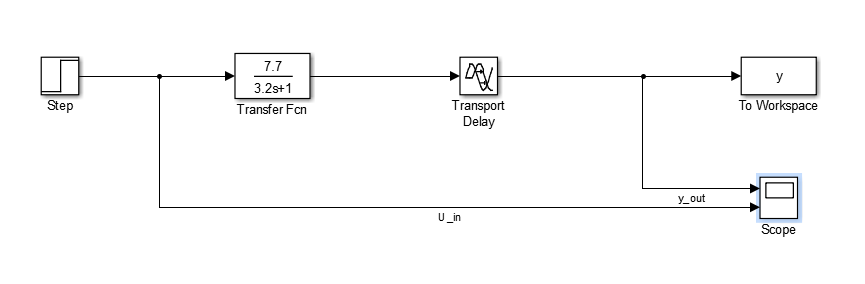
\includegraphics[width=1\linewidth]{images/general/block_dia_simu}
\end{center}
\caption{Block diagram of the simulation}
\label{fig:block_dia_simu}
\end{figure}

\begin{figure}[H]
\begin{center}
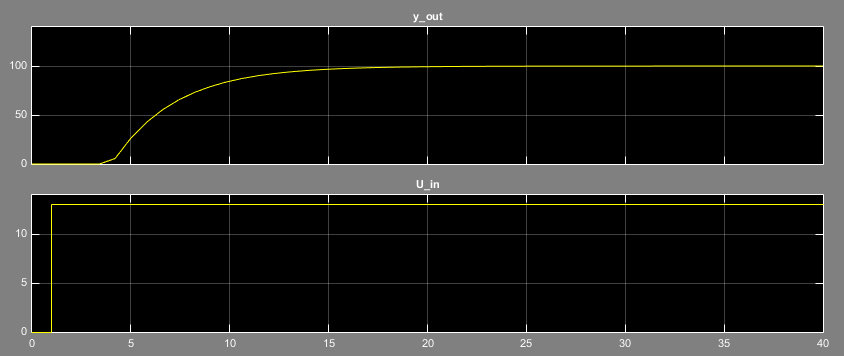
\includegraphics[width=1\linewidth]{images/general/step_resp_simu}
\end{center}
\caption{Step response the system}
\label{fig:step_resp_simu}
\end{figure}